\section{Design}\label{sec:design}
In this section the design of the different parts of the system is designed, based on the system criteria described in section \ref{sec:non-requirements}. These include, but are not limited to, database design, general API design, the smartphone app and the interaction between the different components.

\subsection{Backend}\label{sec:back-end}
The diagram on figure \ref{fig:serversidestructure} describes the overall structure of the backend of the system. The backend contains the web service, accessed through an API.

\begin{figure}[H]
    \centering
    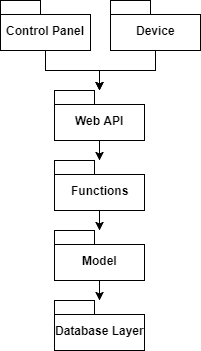
\includegraphics[width=0.35\textwidth]{Figures/serverSide.png}
    \caption{The structure of the backend part of the system}
    \label{fig:serversidestructure}
\end{figure}

The backend of the system is designed as a layered architecture, consisting of a database layer, a model layer, a function layer and the API layer. Each device and the control panel access the features of the web service through the API. Each endpoint of the API has access to the functions that they need, through the function layer, which in turn uses the model layer to interact with data, accessed by the database layer. This design is called an closed-strict design, which only lets upper parts call functionality further down in the layers, and only 1 layer further down. A class-diagram of the model layer can be found on figure \ref{fig:serversidemodel}. 

\begin{figure}[H]
    \centering 
    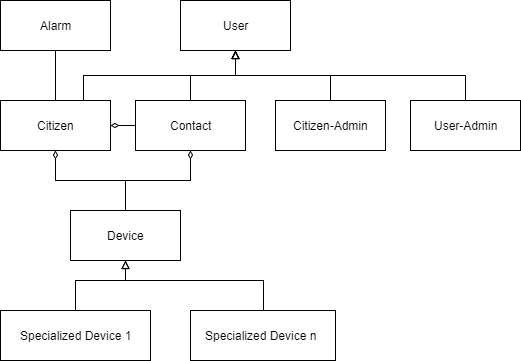
\includegraphics[width=0.9\textwidth]{Figures/serverSidemodel.png}
    \caption{The backend model layer}
    \label{fig:serversidemodel}
\end{figure}

There are several classes in the model, each representing different aspects of the system. There is a super class \textit{User}, which represents a user in the system. Each user type described in section \ref{sec:user-roles} inherits from this super class. Besides the user-related classes, there is also a \textit{Device} and \textit{Alarm} class. Each of these different classes, found on the class diagram \ref{fig:serversidemodel}, and their relationship, are described in details below.

\paragraph{User} is the super class used for all user types in the system. It contains the required login information to access the system, as well as the name of the user.

\paragraph{Citizen} inherits from User. It represents a citizen in the system, and has references to contacts and devices. It also contains information about where the citizen lives, such that the contact can find them when they have fallen.

\paragraph{Contact} inherits from User. It represents a contact in the system, and has references to devices. A contact can exist independently of a citizen, but can not do anything without being connected to a citizen.

\paragraph{Citizen Admin} inherits from User. It represents a user that can create and manage Citizens in the system.

\paragraph{User Admin} inherits from User. The User Admin is an administrator that administrates all users in the system.

\paragraph{Device} is a super class, representing a device in the system, either used by the citizen or contact.

\paragraph{Specialized device} inherits from Device. There can be an arbitrary amount of specialized devices, each representing a different type of device, such as a smartphone app or smart assistant.

\paragraph{Alarm} contains information about an active alarm. It contains information about who triggered the alarm, the current status of the alarm, and who, if any, that has answered the alarm.

\subsection{Web API}
When designing a web API for a service, it is important to consider which architecture to use and how to facilitate the communication to and from the service. Considering the requirements given in section \ref{sec:non-requirements}, the web API should be implemented using REST. REST was chosen, since it fits well with the general architecture of the system and integrates well with devices such as apps and browsers.

\subsubsection{REST}\label{sub:rest}
REST is short for Representational State Transfer. It is based on the HTTP protocol, and allows a client to communicate by using HTTP messages \cite{restapitutorial}\cite{restwikipedia}\cite{restbook}. The requests use an URI to specify what resource to access. 

HTTP request methods, sometimes also called verbs, are used to specify what action the server should perform on a resource. The HTTP protocol covers many methods, but REST limits itself to the four methods described below:

\paragraph{GET} gets a representation of a resource. The use of GET should never have side effects, and multiple calls to get should always give the same result.
\paragraph{DELETE} deletes a resource. Trying to delete a resource that doesn't exist usually results in an error response, such as 404. DELETE is also idempotent, so sending it multiple times does not cause any damage to the rest of the system, should it be sent twice.
\paragraph{POST} creates a new resource. Unlike DELETE, POST is not idempotent, so sending the same request twice will create the resource twice. 
The standard also specifies that the POST method can be overloaded. POST can do any change: DELETE, PUT, PATCH. When overloading POST, there are no protocol semantics it has to follow.
\paragraph{PUT} updates an existing resource. PUT should also be idempotent, as sending the same PUT message multiple times will just update the resource to what it already is. PUT can also be used as POST, if specifying where the system should put the new resource, and if the implementation allows it.

\subsubsection{Rest constrains}
REST has six constraints that has to be fulfilled for a Web-API to be RESTful, these are defined as follows:

\paragraph{Uniform Interface}  There are four principles for a uniform interface:
\begin{itemize}
\item REST is resource based, so all data is sent between server and client using URIs for identification of the specific resource.
\item When a client has a resource, it should also have enough data to modify it and send the modified resource back to the server.
\item Each message should be self-descriptive, meaning the message itself should contain information about how it should be read.
\item REST used HATEOAS.
\end{itemize}

\paragraph{Stateless} A REST implementation is stateless if the server has no knowledge of the state of the client. All relevant data for the state of the client has to be sent to the server at each call, and nothing is kept between calls.

\paragraph{Cacheable} Some responses can be cached, while others cannot. So a resource must know if it can become stale between uses.

\paragraph{Client-Server} Clients should not be concerned with storage of data, while the server should not be concerned with user interface or user state. As long as the interface between server and client is unaltered, they can be developed independently.

\paragraph{Layered System} A client cannot tell if it is talking to the endpoint, or an intermediary. This allows load-balancing as multiple intermediary servers can run on multiple physical units, and still connect to the same end-point.

\paragraph{Code on Demand} The server can extend its functionality by sending logic that can be executed by the client. This step is unlike the others optional for an API to be RESTful.

The system will follow the above constrains where possible, but there will be exceptions. Information cannot be cached since alarms needs to always be up to date, and since an accident can happen immediately after changing info or devices, that can not be changed either. The client and server should send models where possible, that represent the state of the system.

\subsection{Control panel}
The diagram shown on \ref{fig:controlpanel} describes the different views in the control panel. 

\begin{figure}[H]
    \centering
    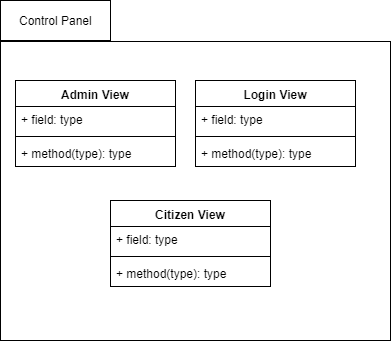
\includegraphics[width=0.4\textwidth]{Figures/ControlPanel.png}
    \caption{The different views included in the control panel}
    \label{fig:controlpanel}
\end{figure}\todo{Ret admin view til register view}

The login view is the first view shown, when a user accesses the interface. This view allows them to login to the system and gives access to the rest of the views.

The register view can be accessed from the login view. The register view is used to add new users of role citizen and contact.

The citizen view is for users with citizen admin rights. The view will show the information on all the citizen the citizen admin is administrating and allow them to add to these or edit the existing.

\subsection{Smartphone app}
The smartphone app is one of the components where interaction with the citizens takes place. It is designed as an app and an underlying fall detection service, which then interacts with the web service, using the web API.

\begin{figure}[H]
    \centering
    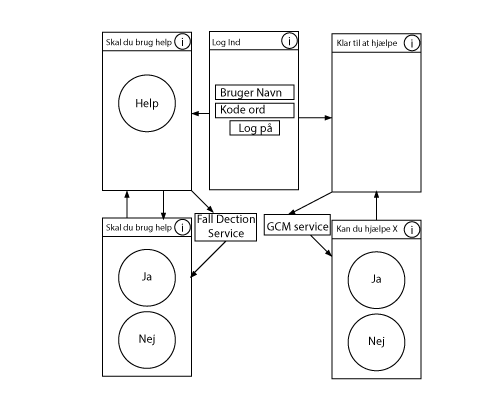
\includegraphics[width=1.0\textwidth]{Figures/MobilUI.png}
    \caption{Prototype of smartphone UI}
    \label{fig:mobilUI}
\end{figure}

Figure \ref{fig:mobilUI} shows an early low fidelity prototype of the app. It illustrates both the flow through the views and their individual designs, the views are numbered 1 to 5 in red. This is not part of the app, but has been added to make it possible to reference each view.

View 1 is the first view that the user meets. Here the user can login. The app then changes to either View 2 or View 4, depending on the type of user that is returned from the web service.

View 2 consists of a button to call for help, which, when clicked will change to view 3. In view 3, the citizen has to confirm whether or not they have fallen, either verbally or by physically clicking one of the buttons. If no input is given, the view will time out and call for help. This view is also shown when the apps fall detection service detects a fall. The fall detection service is running even when the app is not.

View 4 is reached when logging in as a contact. A contact will only leave this view when they receive an alarm from an associated citizen. This alarm will come in the form of a notification. When the contact reacts to the notification, they are taken to view 5 where the name of the citizen in need of help, is shown. The contact must then whether or net they are able to help the citizen. The app then sends this response to the web service.

\subsection{Communication}
In this section, sequence diagrams are presented to better understand how the different devices communicate with, and through the web service, using the API. These are different from the diagrams found in section \ref{sec:system-behaviour}, since these show how the different components communicate, where as the ones described earlier show how the different actors, with the system being one, interacts with each other. 

Each diagram describes the communication during a specific event.

\begin{figure}[H]
    \centering
    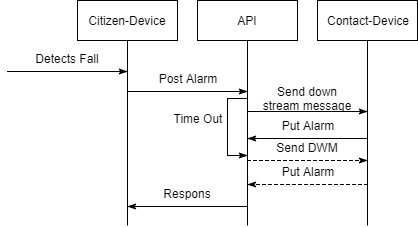
\includegraphics[width=0.7\textwidth]{Figures/Citizen_to_Contact.png}
    \caption{Communication between devices during an alarm activation}
    \label{fig:post-alarm}
\end{figure}

When a citizens device detects a fall, as described in section \ref{sec:system-behaviour}, it posts an \textit{Alarm} to the web API.
Figure \ref{fig:post-alarm} shows how a citizens device posts an alarm to the web service and how the web service reacts.

The notification contains enough information such that the contact can update the alarm, with information about whether or not they can help.

\begin{figure}[H]
    \centering
    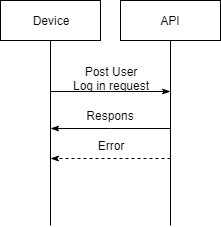
\includegraphics[width=0.4\textwidth]{Figures/Device-Api.png}
    \caption{Communication between devices during sign-in}
    \label{fig:post-sign-in}
\end{figure}

During a \textit{login} event, the system reacts as seen on figure \ref{fig:post-sign-in}. If the request is successful, the web service will return the corresponding user. If not, it returns an error. The returned user should contain enough info such that any system that tries to login, is able to operate on the data without the need to request further data on the user.

Any call made to the web API should happen to specific endpoints that each have their own area of responsibility.

\begin{figure}[H]
    \centering
    \begin{itemize}
        \item User
        \begin{itemize}
            \item Create a new user
            \item Edit an existing
            \item Log in to an existing user
            \item Delete a user
        \end{itemize}
        \item Citizen
        \begin{itemize}
            \item Get a specific citizen
            \item Get all citizens
            \item Add a device to a citizen
            \item Add a contact to a citizen
        \end{itemize}
        \item Contact
        \begin{itemize}
            \item Get a specific Contact
            \item Get all Contact
            \item Add a device to a Contact
        \end{itemize}
        \item Alarm
        \begin{itemize}
            \item Create a new alarm for a citizen
            \item Update an existing alarm
            \item Get an existing alarm
            \item Stop an alarm.
        \end{itemize}
    \end{itemize}
    \caption{API endpoints}
    \label{fig:design_endpoint}
\end{figure}

Figure \ref{fig:design_endpoint} gives an overview of the different endpoints the API should have and what they should do. The API should be structured in a way such that it follows the rules for REST as described in section \ref{sub:rest}. The endpoints allow for all the interactions that should be needed in the model.

\subsection{Database design}\label{sec:databasedesign}
To get a better understanding of the design of the database, used in this project, an ER diagram is shown on figure \ref{fig:database}.

\begin{figure}[H]
    \centering
    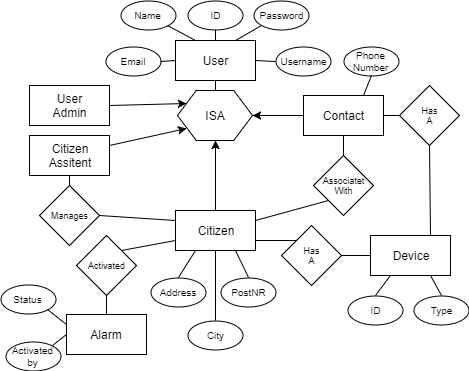
\includegraphics[width=1.0\textwidth]{Figures/Database.png}
    \caption{Database design}
    \label{fig:database}
\end{figure}

The database design consists of seven entities, where four of these are specifications of the \textit{User} entity. These specifications are \textit{Citizen}, \textit{Contact}, \textit{Citizen admin} and \textit{User admin}, and represents the different user types that exists in the system, as described in section \ref{sec:back-end}. 

The last two entities are \textit{Alarm} and \textit{Device}. The \textit{Alarm} entity represents an alarm in the system, it has a foreign key \textit{Activated by} that points to the citizen who has activated the alarm and a status property that represents the current state of the alarm. The \textit{Device} entity represents the devices that citizens and contacts has.